\documentclass[conference]{IEEEtran}
\usepackage[utf8]{inputenc}
\usepackage[T1]{fontenc}
\usepackage[spanish,es-tabla]{babel}
\usepackage{amsmath,amssymb}
\usepackage{graphicx}
\usepackage{booktabs}
\usepackage{array}
\usepackage{tabularx}
\usepackage{float}      % habilita [H]: la figura/tabla queda exactamente donde se escribe
\usepackage{siunitx}
\usepackage{listings}
\usepackage{xcolor}
\usepackage{hyperref}

\sisetup{output-decimal-marker={.}}
\lstset{basicstyle=\ttfamily\footnotesize, breaklines=true, frame=single, language=C}

% Columnas para tabularx: X = ajusta al ancho disponible y parte líneas
\newcolumntype{L}{>{\raggedright\arraybackslash}X}   % texto a la izquierda
\newcolumntype{C}{>{\centering\arraybackslash}X}     % texto centrado
\renewcommand{\arraystretch}{1.15}

% REGLAS DE LA PLANTILLA
% - Toda tabla usa tabularx con ancho \columnwidth: nunca se sale de la columna.
% - Toda figura y tabla usa [H]: aparece justo donde se instancia en el código.
% - Las imágenes van con width=\columnwidth (o menos).

\begin{document}

\title{MARLUP: Actividad 3 -- Desarrollo de sistema\\Processor-in-the-Loop}

\author{
\IEEEauthorblockN{Aarón Salas Alvarado, Mónica Solís Murillo, Eduardo Valle Arriola}
\IEEEauthorblockA{Instituto Tecnológico de Costa Rica\\
% Curso y profesor
}
}

\maketitle

% =====================================================================
% 150--200 palabras: qué se hizo, resultado principal con números,
% causa principal de la degradación.
\begin{abstract}
MARLUP es una plataforma de nivelación accionada por cilindros hidráulicos. Este trabajo valida su controlador de posición mediante un esquema \textit{Processor-in-the-Loop} (PiL). El modelo dinámico de un actuador, compuesto por un cilindro Bosch Rexroth CDH1 40/28 y una válvula proporcional 4/3, se simula en Simulink. El controlador PI, sintonizado manualmente ($K_p=60$, $K_i=1$, saturación en $\pm1$) y discretizado por Tustin con $T_s=\SI{10}{ms}$, se ejecuta en un Arduino UNO R3 mediante el flujo \textit{Processor-in-the-Loop} de Simulink: Embedded Coder genera el código C del controlador, lo compila y lo carga en la placa, y un bloque Model en modo PIL intercambia la posición y el comando con ella por UART. Se realizaron dos implementaciones. En la primera, sensores y actuadores son ideales; en la segunda, se incorporan no idealidades tomadas de las hojas de datos: cuantización del ADC, error de linealidad e histéresis del sensor magnetostrictivo. El PiL ideal reproduce exactamente la simulación MiL (error nulo en las 401 muestras), mientras que el caso no ideal alcanza un sobreimpulso de \SI{3.47}{\percent} y un error en estado estacionario de \SI{0.047}{mm}, frente al requisito de \SI{2.3}{mm}. La degradación se atribuye principalmente a la cuantización del ADC, que por sí sola produce un error RMS de \SI{0.121}{mm} respecto al MiL.
\end{abstract}

\begin{IEEEkeywords}
Processor-in-the-Loop, control hidráulico, controlador discreto, no idealidades, MARLUP.
\end{IEEEkeywords}

% =====================================================================
\section{Introducción}
% Alcance del PiL (una pata / tres patas) y objetivo específico 5 del Avance 2.
% Requisitos: Mp < 10 %, error de nivelación < 0.2° (~2.3 mm).
MARLUP es una plataforma de nivelación que controla el \textit{roll} y el \textit{pitch} de su mesa mediante cilindros hidráulicos, de forma similar a las plataformas paralelas de compensación de movimiento \cite{wang2025}. En la etapa anterior se diseñó, sobre un modelo dinámico del actuador, un controlador PI de posición que cumple los requisitos de sobreimpulso menor al \SI{10}{\percent} y error de nivelación menor a \SI{0.2}{\degree}, equivalente a unos \SI{2.3}{mm} de elongación del cilindro.

Un controlador validado solo en simulación (\textit{Model-in-the-Loop}, MiL) no considera los efectos del hardware: la discretización, la resolución finita del ADC y del PWM, y la latencia de comunicación. Este trabajo evalúa esos efectos mediante un esquema \textit{Processor-in-the-Loop} (PiL). El modelo de un actuador se ejecuta en Simulink y el controlador se ejecuta en un Arduino UNO R3; ambos se comunican por UART. Se comparan tres casos: MiL, PiL con sensores y actuadores ideales, y PiL con no idealidades tomadas de las hojas de datos.
% =====================================================================
\section{Modelo de planta en Simulink}
\label{sec:planta}
% Resumen del modelo hidráulico remitiendo al Avance 2 y reajuste del MiL.

El modelo dinámico del actuador parte del descrito en \cite{avance2}. Está compuesto por una válvula direccional proporcional 4/3, un cilindro de doble efecto Bosch Rexroth CDH1 40/28 \cite{rexroth}, tuberías de \SI{16}{mm} de diámetro y \SI{0.8}{m} de longitud, y una masa móvil con fricción viscosa. Sus parámetros se resumen en la Tabla~\ref{tab:planta}. La posición $x$ se mide desde el vástago totalmente retraído ($x=0$).

Respecto a \cite{avance2}, el MiL se reajustó. Con la sintonización original ($K_p=6.7$, $K_i=1$), la válvula solo saturaba para errores mayores a \SI{0.15}{m}, y la acción integral, con una constante de tiempo cercana a \SI{7}{s}, producía una cola de asentamiento de unos \SI{12}{s}. Por ello se elevó $K_p$ a 60, manteniendo $K_i=1$, y se limitó el comando a $u\in[-1,1]$, el rango normalizado de apertura de la válvula. Además, se aumentaron la presión de suministro a \SI{160}{bar} y el caudal nominal de la válvula a \SI{40}{L/min}. Con $K_p=60$, la válvula permanece abierta casi todo el recorrido y empieza a cerrar a unos \SI{1.7}{cm} ($1/K_p$) del objetivo. La frecuencia natural hidráulica estimada es $\omega_h\approx\SI{390}{rad/s}$, con $\zeta\approx0.06$.

La presión de suministro queda por debajo de la nominal del cilindro (\SI{250}{bar}), y la velocidad máxima alcanzada, de aproximadamente \SI{0.40}{m/s}, queda por debajo de su límite de \SI{0.5}{m/s} \cite{rexroth}. Para un escalón de \SIrange{0}{0.40}{m} aplicado en $t=\SI{0.5}{s}$, que deja \SI{5}{cm} de margen al tope de carrera, el MiL con el controlador discreto de la Sec.~\ref{sec:control} presenta un tiempo de subida de \SI{0.73}{s}, un tiempo de asentamiento al \SI{2}{\percent} de \SI{1.05}{s} y un sobreimpulso de \SI{3.43}{\percent} (\SI{13.7}{mm}), con un error en estado estacionario de \SI{0.014}{mm}.

\begin{table}[H]
\centering
\caption{Parámetros del modelo de planta}
\label{tab:planta}
\small
\begin{tabularx}{\columnwidth}{Ll}
\toprule
Parámetro & Valor \\
\midrule
Cilindro \cite{rexroth} & CDH1 40/28 \\
Área del pistón $A_1$ & \SI{12.57}{cm^2} \\
Área anular $A_3$ & \SI{6.41}{cm^2} \\
Carrera $L_{cyl}$ & \SI{0.45}{m} \\
Posición inicial $x_0$ & \SI{0}{m} (retraído) \\
Presión de suministro $p_s$ & \SI{160}{bar} \\
Módulo volumétrico efectivo $\beta_e$ & \SI{750}{MPa} \\
Masa móvil $m$ & \SI{20}{kg} \\
Fricción viscosa $b$ & \SI{1000}{N\,s/m} \\
Tuberías (diámetro, longitud) & \SI{16}{mm}, \SI{0.8}{m} \\
Caudal nominal de la válvula $Q_N$ & \SI{40}{L/min} a \SI{35}{bar} \\
Constante de tiempo de la válvula $\tau_v$ & \SI{2}{ms} \\
Retardo de la válvula $T_d$ & \SI{1}{ms} \\
\bottomrule
\end{tabularx}
\end{table}

% =====================================================================
\section{Arquitectura PiL y comunicación}
\label{sec:arq}

\subsection{Hardware y software}
% MCU, reloj, versión de MATLAB/Simulink, puerto y baudios.
La planta se simula en MATLAB/Simulink R2026a con un solver de paso fijo \texttt{ode4} de \SI{0.1}{ms}. El controlador se ejecuta en un Arduino UNO R3 (ATmega328P, \SI{16}{MHz}) conectado por USB (puerto COM6) mediante el flujo \textit{Processor-in-the-Loop} de Simulink, con Embedded Coder y el \textit{Simulink Support Package for Arduino Hardware}. La Fig.~\ref{fig:arq} resume el lazo: la planta, el modelo del sensor y la referencia están en Simulink, y la ley de control, en el MCU.

\begin{figure}[H]
\centering
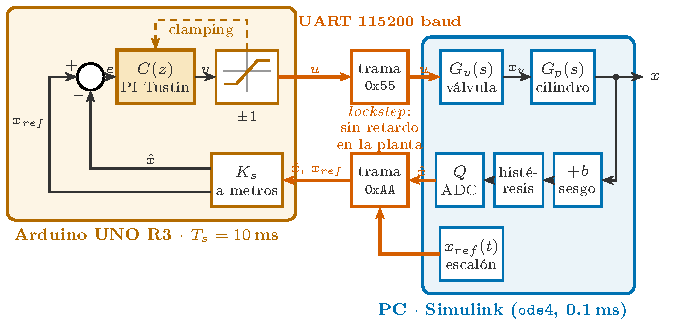
\includegraphics[width=\columnwidth]{figuras/arquitectura_pil.pdf}   % fuente: figuras/arquitectura_pil.tex
\caption{Arquitectura PiL: planta y modelo del sensor en Simulink, controlador en el MCU.}
\label{fig:arq}
\end{figure}

\subsection{Modelos en Simulink y comunicación}
\label{sec:pil_oficial}
El controlador está en el modelo \texttt{ctrl\_pi.slx} (Fig.~\ref{fig:simctrl}): un bloque Discrete PID Controller en forma PI, con integrador trapezoidal (Tustin), $K_p=60$, $K_i=1$, $T_s=\SI{10}{ms}$, saturación en $\pm1$ y anti-windup por \textit{clamping}, es decir, la ley \eqref{eq:pi}. Este modelo se referencia desde \texttt{PiL.slx} (Fig.~\ref{fig:simpil}) con un bloque Model. En modo PIL, Embedded Coder genera el código C de \texttt{ctrl\_pi}, lo compila para el ATmega328P y lo carga en la placa. En cada periodo $T_s$, Simulink envía por el puerto serie (\SI{115200}{baud}) la referencia y la posición medida, el MCU ejecuta un paso del código generado y devuelve $u[k]$. La simulación queda así sincronizada paso a paso con el MCU (\textit{lockstep}): Simulink no avanza hasta recibir $u[k]$, por lo que la latencia de la comunicación no se traslada a la planta. Con el mismo bloque en modo Normal, el controlador se simula en el PC y constituye la referencia MiL. Como en el AVR un \texttt{double} ocupa 4 bytes, la interfaz del controlador es de precisión simple y el modelo host convierte los tipos a la entrada y a la salida. Las no idealidades del sensor (Sec.~\ref{sec:noideal}) son bloques de Simulink en el camino de realimentación: sesgo, histéresis (\textit{backlash}), cuantización y rango del ADC.

% A doble columna para que el diagrama sea legible (figure* no admite [H])
\begin{figure*}[t]
\centering
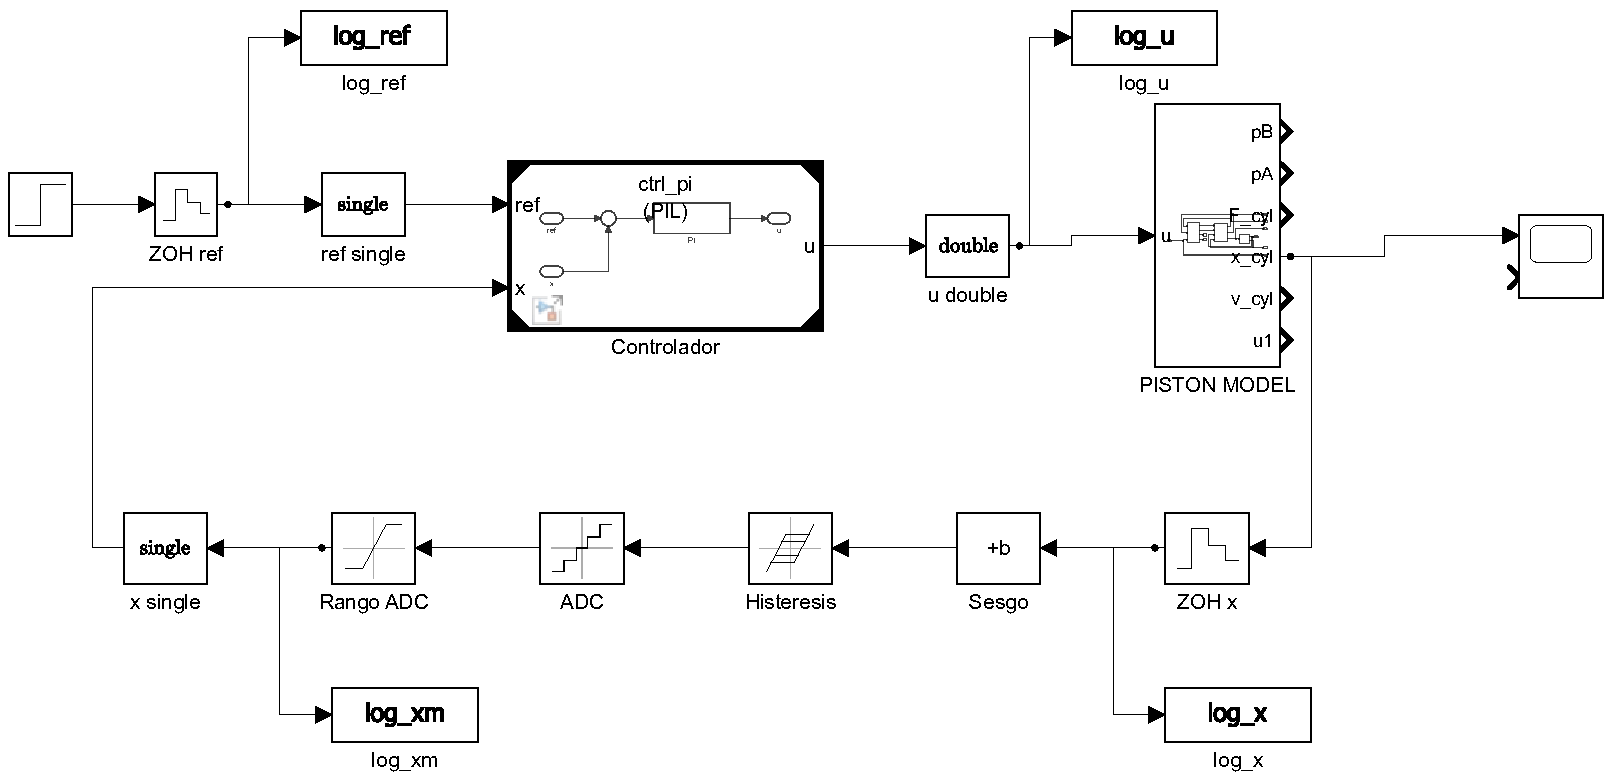
\includegraphics[width=0.85\textwidth]{figuras/simulink_pil.pdf}
\caption{Modelo \texttt{PiL.slx}: el bloque Controlador referencia \texttt{ctrl\_pi} en modo PIL; abajo, el modelo del sensor con sus no idealidades.}
\label{fig:simpil}
\end{figure*}

\begin{figure}[H]
\centering
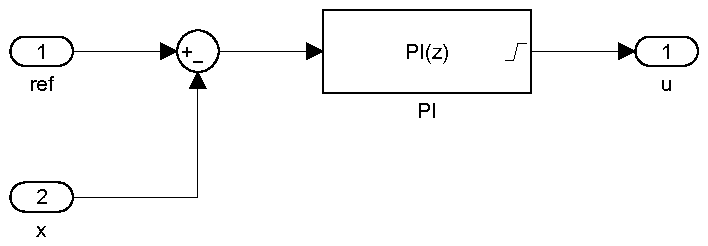
\includegraphics[width=0.75\columnwidth]{figuras/simulink_ctrl_pi.pdf}
\caption{Modelo \texttt{ctrl\_pi.slx}, compilado y ejecutado en el Arduino UNO R3.}
\label{fig:simctrl}
\end{figure}



% =====================================================================
\section{Interfaz sensor/actuador -- MCU}
\label{sec:interfaz}

\subsection{Sensor de posición}
% mm -> V -> bits ADC -> cuentas; resolución en mm/cuenta vs 2.3 mm.
La posición se mide con el sensor magnetostrictivo integrado en el cilindro CDH1, de salida analógica \SIrange{0}{10}{V} \cite{rexroth}. Un divisor 1:2 adapta esta señal al ADC de 10 bits del Arduino (\SI{5}{V}), cuya resolución en posición es
\begin{equation}
\Delta x = \frac{L_{cyl}}{2^{N}} = \frac{\SI{450}{mm}}{1024} \approx \SI{0.44}{mm},
\label{eq:resolucion}
\end{equation}
muy por debajo del error de nivelación admisible de \SI{2.3}{mm}.

\subsection{Electroválvula}

Como actuador se usa la válvula proporcional 4/3 Bosch Rexroth 4WREE~6 en su versión de \SI{32}{L/min} (a \SI{10}{bar} por arista de control), compatible con el caudal nominal de \SI{40}{L/min} a \SI{35}{bar} del modelo. La válvula recibe un comando de $\pm\SI{10}{V}$ \cite{rexroth_4wree}. El Arduino genera $u$ como un PWM de 8 bits centrado ($D=\SI{50}{\percent}+\SI{50}{\percent}\cdot u$), que un filtro RC y un amplificador llevan a $V_{cmd}=\SI{10}{V}\cdot u$. La resolución del comando es $\Delta u=2/256\approx0.0078$ y, con la saturación en $\pm1$, se usa el rango completo de 256 cuentas. Con $K_p=60$, un paso del ADC (\SI{0.44}{mm}) equivale a un cambio de 0.026 en $u$, unas tres cuentas del PWM, por lo que la cuantización de la medición se refleja directamente en el comando.
\begin{table}[H]
\centering
\caption{Cadena de conversión de señales en el Arduino UNO R3}
\label{tab:interfaz}
\small
\begin{tabularx}{\columnwidth}{lL}
\toprule
Etapa & Conversión \\
\midrule
\multicolumn{2}{l}{\textbf{Medición de posición} (pistón $\rightarrow$ Arduino)} \\
Sensor del cilindro & \SIrange{0}{450}{mm} $\rightarrow$ \SIrange{0}{10}{V} \\
Divisor 1:2 & \SIrange{0}{10}{V} $\rightarrow$ \SIrange{0}{5}{V} \\
ADC 10 bits & \SIrange{0}{5}{V} $\rightarrow$ 0 a 1023 cuentas \\
\textit{Resolución} & \textit{\SI{0.44}{mm} por cuenta} \\
\midrule
\multicolumn{2}{l}{\textbf{Comando de la válvula} (Arduino $\rightarrow$ válvula)} \\
Controlador PI & $u \in [-1,\,1]$ \\
PWM 8 bits, \SI{490}{Hz} & $u \rightarrow$ ciclo de trabajo de 0 a \SI{100}{\percent} \\
Filtro RC & ciclo de trabajo $\rightarrow$ \SIrange{0}{5}{V} \\
Amplificador & \SIrange{0}{5}{V} $\rightarrow$ $\pm\SI{10}{V}$ \\
\textit{Resolución} & \textit{$\Delta u = 2/256 \approx 0.0078$} \\
\bottomrule
\end{tabularx}
\end{table}




\section{Implementación del controlador en hardware}
\label{sec:control}

El controlador se ejecuta en un Arduino UNO R3 \cite{arduino_uno}, basado en el microcontrolador ATmega328P de 8 bits a \SI{16}{MHz} \cite{atmega328p}. El PI, sintonizado manualmente ($K_p=60$, $K_i=1$), se discretizó por el método de Tustin con un periodo de muestreo $T_s=\SI{10}{ms}$ y se implementó en forma posicional:
\begin{equation}
\begin{aligned}
I[k] &= I[k-1] + \tfrac{K_iT_s}{2}\big(e[k]+e[k-1]\big),\\
u[k] &= \operatorname{sat}_{\pm1}\!\big(K_p\, e[k] + I[k]\big),
\end{aligned}
\label{eq:pi}
\end{equation}
con anti-windup por \textit{clamping}: la integral no se actualiza cuando el comando está saturado y el error empuja en el mismo sentido de la saturación. Se descartó la forma incremental $u[k]=\operatorname{sat}(u[k-1]+q_0e[k]+q_1e[k-1])$. Con un escalón de \SI{0.40}{m}, la acción proporcional ($K_p e\approx24$) se recorta a 1 en la primera muestra y esa forma ``olvida'' el resto: el comando cae a cero cuando el pistón avanza $1/K_p\approx\SI{1.7}{cm}$, y a partir de ahí solo la integral, lenta, mueve el pistón. En el MiL, con esa forma, el pistón llegó apenas a \SI{38}{mm} en \SI{3.5}{s}. La ley se implementa con el bloque Discrete PID Controller de Simulink y Embedded Coder genera a partir de él el código C que corre en el MCU, en aritmética de punto flotante de 32 bits. El periodo de muestreo lo impone Simulink: el código generado ejecuta un paso cada vez que recibe las entradas de un periodo, por lo que el lazo queda sincronizado sin requerir un temporizador propio en el MCU.

El periodo $T_s=\SI{10}{ms}$ es mucho menor que el tiempo de asentamiento del lazo (\SI{1.05}{s}). En cambio, la resonancia hidráulica estimada ($\omega_h\approx\SI{390}{rad/s}$, unos \SI{62}{Hz}) queda por encima de la frecuencia de Nyquist ($f_s/2=\SI{50}{Hz}$); si se excitara, aparecería en la medición como un alias cercano a \SI{38}{Hz}. Como la válvula opera saturada durante casi todo el recorrido y el frenado es suave, no se espera excitarla; esto se verifica en los resultados.




\newpage
%De aqui en adelante no  tengo nada
% =====================================================================
\section{Implementación 1: sensores y actuadores ideales}
\label{sec:ideal}
% Escalón 0 -> 0.40 m. RMSE y error máximo MiL vs PiL.
Se aplicó un escalón de referencia de \SIrange{0}{0.40}{m} en $t=\SI{0.5}{s}$ y se simularon \SI{4}{s}. En el PiL ideal, la posición se envía al MCU sin modelo de sensor; la única diferencia con el MiL es que el controlador corre como código C generado en el ATmega328P en lugar de simularse en el PC. La Fig.~\ref{fig:ideal} compara ambas respuestas: en las 401 muestras de la corrida, la posición y el comando del PiL ideal coinciden exactamente con los del MiL (error RMS y error máximo nulos). Esto confirma que el código generado reproduce bit a bit la simulación del controlador en precisión simple y que el intercambio con el MCU, en \textit{lockstep}, no introduce diferencias.

\begin{figure}[H]
\centering
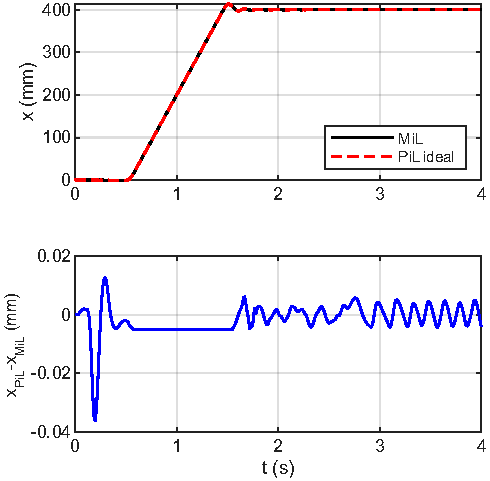
\includegraphics[width=\columnwidth]{figuras/mil_vs_pil_ideal.pdf}
\caption{Respuesta al escalón de \SIrange{0}{0.40}{m}: MiL y PiL ideal.}
\label{fig:ideal}
\end{figure}

% =====================================================================
\section{Implementación 2: sensores y actuadores no ideales}
\label{sec:noideal}
% Al menos 3 no idealidades nuevas, con fuente. Una corrida por cada una y todas juntas.

Se implementaron tres no idealidades en el modelo del sensor, del lado de Simulink, con los bloques Bias, Backlash, Quantizer y Saturation (Fig.~\ref{fig:simpil}), en el orden sesgo, histéresis (\textit{backlash}) y cuantización, de modo que el MCU recibe la posición tal como la entregaría el ADC. Los valores del sensor se tomaron de la hoja de datos del fabricante \cite{rexroth} y se refieren a la carrera $L_{cyl}=\SI{0.45}{m}$. El error de linealidad es de $\pm\SI{0.02}{\percent}$ de la longitud de medición, es decir, $\pm\SI{0.09}{mm}$, y se modela en el peor caso como un sesgo constante. La histéresis es de \SI{0.004}{mm}. La cuantización sigue \eqref{eq:resolucion} y es la no idealidad de medición de mayor magnitud. La repetibilidad del sensor ($\pm\SI{0.0045}{mm}$) es dos órdenes de magnitud menor que la cuantización y no se modela. El límite de velocidad del fabricante (\SI{0.5}{m/s}) tampoco se incluye, ya que, como se mostró en la Sec.~\ref{sec:planta}, la velocidad máxima del MiL es de aproximadamente \SI{0.40}{m/s}. Se realizó una corrida con cada no idealidad por separado y una con las tres juntas.

\begin{table}[H]
\centering
\caption{No idealidades implementadas}
\label{tab:noideal}
\small
\begin{tabularx}{\columnwidth}{LlcL}
\toprule
No idealidad & Valor & Fuente & Modelo \\
\midrule
Cuantización ADC & $L_{cyl}/2^N$ & \cite{atmega328p} & Redondeo a 1024 niveles \\
Error de linealidad & $+\SI{0.09}{mm}$ & \cite{rexroth} & Sesgo constante \\
Histéresis del sensor & \SI{0.004}{mm} & \cite{rexroth} & Banda muerta (\textit{backlash}) \\
\bottomrule
\end{tabularx}
\end{table}

% =====================================================================
\section{Resultados y análisis comparativo}

\subsection{Respuesta MiL vs PiL ideal vs PiL no ideal}
La Fig.~\ref{fig:comparacion} muestra la posición y el comando en los tres casos. Durante el recorrido, las tres curvas son indistinguibles: la válvula queda saturada en $u=1$ desde el escalón hasta que el error baja de $1/K_p$, el pistón avanza a velocidad casi constante y el frenado produce el mismo sobreimpulso y las mismas oscilaciones amortiguadas. Esas oscilaciones son lentas, de pocos ciclos entre \SI{1.5}{s} y \SI{2}{s}, y en $u$ no aparece ninguna componente rápida que indique el alias de la resonancia hidráulica discutido en la Sec.~\ref{sec:control}. Las diferencias solo se aprecian en el detalle cerca de la referencia: el PiL ideal se superpone al MiL, mientras que el PiL no ideal mantiene una pequeña oscilación sostenida alrededor de \SI{400}{mm} y queda ligeramente por debajo de la referencia.

\begin{figure}[H]
\centering
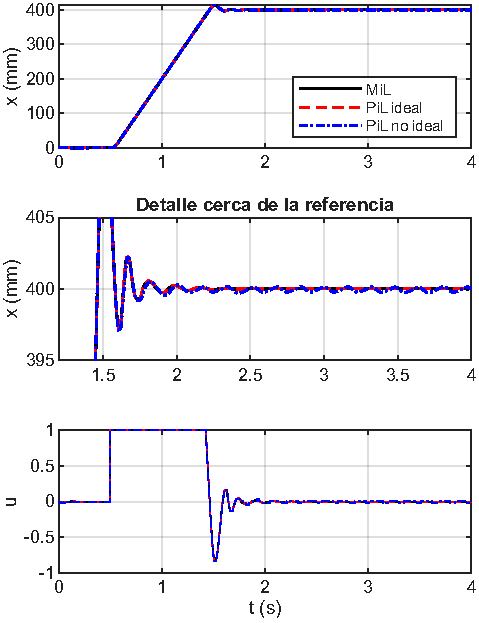
\includegraphics[width=\columnwidth]{figuras/comparacion_x_u.pdf}
\caption{Posición y comando de control en los tres casos.}
\label{fig:comparacion}
\end{figure}

\subsection{Métricas de desempeño}
La Tabla~\ref{tab:metricas} resume las métricas de los tres casos, calculadas desde el escalón ($t\geq\SI{0.5}{s}$); el error en estado estacionario es el promedio del error en el último segundo. El tiempo de subida (\SI{0.73}{s}) y el de asentamiento (\SI{1.05}{s}) coinciden en los tres casos con la resolución de $T_s$, y el RMS del comando es 0.528 en todos ellos, porque el recorrido está dominado por la saturación. El PiL ideal coincide exactamente con el MiL en todas las métricas: $M_p=\SI{3.43}{\percent}$ y $e_{ss}=\SI{0.014}{mm}$. En el PiL no ideal el sobreimpulso sube a \SI{3.47}{\percent} (\SI{13.88}{mm}) y el error en estado estacionario a \SI{0.047}{mm}, con un error RMS de \SI{0.160}{mm} y un error máximo de \SI{0.521}{mm} respecto al MiL.

\begin{table}[H]
\centering
\caption{Métricas de desempeño}
\label{tab:metricas}
\small
\begin{tabularx}{\columnwidth}{lcCCC}
\toprule
Métrica & Req. & MiL & PiL ideal & PiL no ideal \\
\midrule
$M_p$ (\%) & $<10$ & 3.43 & 3.43 & 3.47 \\
$t_r$ (s) & -- & 0.73 & 0.73 & 0.73 \\
$t_s$ 2\,\% (s) & -- & 1.05 & 1.05 & 1.05 \\
$e_{ss}$ (mm) & $<2.3$ & 0.014 & 0.014 & 0.047 \\
RMS($u$) & -- & 0.528 & 0.528 & 0.528 \\
RMSE vs MiL (mm) & -- & -- & 0 & 0.160 \\
$e_{\max}$ vs MiL (mm) & -- & -- & 0 & 0.521 \\
\bottomrule
\end{tabularx}
\end{table}

\subsection{Análisis de la degradación}
% MiL -> PiL ideal; PiL ideal -> no ideal (cuál domina); cumplimiento con márgenes.
El paso de MiL a PiL ideal no introduce ninguna diferencia: error nulo en las 401 muestras. Como la simulación corre en \textit{lockstep}, la latencia de la UART no llega a la planta, y como el MiL ya simula el controlador en precisión simple, la aritmética de 32 bits del AVR tampoco produce diferencias. El código generado es, por tanto, una implementación fiel del controlador diseñado, y toda la degradación del caso no ideal proviene de la medición.

La Tabla~\ref{tab:degradacion} y la Fig.~\ref{fig:noideal} separan el aporte de cada no idealidad. La cuantización del ADC es la causa principal de la degradación: por sí sola produce un error RMS de \SI{0.121}{mm} y un error máximo de \SI{0.256}{mm} respecto al MiL, y genera la oscilación sostenida alrededor de la referencia, de amplitud menor a un paso del ADC (\SI{0.44}{mm}). El error de linealidad le sigue con \SI{0.089}{mm} RMS, pero domina el error en estado estacionario (\SI{0.076}{mm}): como el PI regula la posición medida, la posición real tiende a quedar desplazada en el sesgo de \SI{0.09}{mm}, y la integral, con $K_i=1$, aún no lo alcanza a los \SI{4}{s}. La histéresis de \SI{0.004}{mm} es despreciable (\SI{0.0048}{mm} RMS, $e_{ss}=\SI{0.014}{mm}$, igual al ideal). Los efectos no se suman linealmente: con las tres juntas, el error RMS es de \SI{0.160}{mm} y el error máximo de \SI{0.521}{mm}, pero el $e_{ss}$ (\SI{0.047}{mm}) es menor que con el sesgo solo: como el sesgo (\SI{0.09}{mm}) es una fracción del paso del ADC (\SI{0.44}{mm}), el redondeo enmascara parte de él.

Aun en el caso no ideal, el controlador cumple ambos requisitos con amplio margen: $M_p=\SI{3.47}{\percent}$ frente al límite de \SI{10}{\percent} (margen de \num{6.53} puntos porcentuales) y $e_{ss}=\SI{0.047}{mm}$ frente a \SI{2.3}{mm} (margen de \SI{2.25}{mm}, unas 49 veces por debajo del límite).

\begin{table}[H]
\centering
\caption{Aporte de cada no idealidad (PiL, una por corrida)}
\label{tab:degradacion}
\small
\begin{tabularx}{\columnwidth}{lCCCC}
\toprule
Caso & $M_p$ (\%) & $e_{ss}$ (mm) & RMSE (mm) & $e_{\max}$ (mm) \\
\midrule
Ideal & 3.43 & 0.014 & 0 & 0 \\
Cuantización & 3.41 & 0.024 & 0.121 & 0.256 \\
Linealidad & 3.40 & 0.076 & 0.089 & 0.092 \\
Histéresis & 3.42 & 0.014 & 0.0048 & 0.0098 \\
Todas & 3.47 & 0.047 & 0.160 & 0.521 \\
\bottomrule
\end{tabularx}
\end{table}

\begin{figure}[H]
\centering
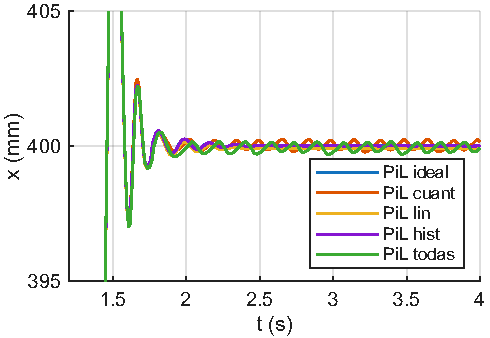
\includegraphics[width=\columnwidth]{figuras/no_idealidades_detalle.pdf}
\caption{Detalle de la posición cerca de la referencia para cada no idealidad por separado y para las tres juntas.}
\label{fig:noideal}
\end{figure}

% =====================================================================
\section{Conclusiones}
\label{sec:conclusiones}
% 3--4 conclusiones con número, limitaciones y trabajo futuro.
\begin{itemize}
\item El código C generado por Embedded Coder y ejecutado en el ATmega328P reproduce exactamente la simulación MiL del controlador: error nulo en las 401 muestras, con $M_p=\SI{3.43}{\percent}$ y $e_{ss}=\SI{0.014}{mm}$ en ambos casos.
\item El flujo PIL de Simulink compila, carga y ejecuta el controlador en la placa sin modificar el modelo de diseño; solo exige una interfaz en precisión simple, porque en el AVR un \texttt{double} ocupa 4 bytes.
\item La cuantización del ADC de 10 bits es la no idealidad dominante (\SI{0.121}{mm} RMS frente a \SI{0.089}{mm} del error de linealidad y \SI{0.0048}{mm} de la histéresis), mientras que el error de linealidad es el que más eleva el error en estado estacionario (\SI{0.076}{mm}).
\item Con todas las no idealidades, el sistema cumple los requisitos con amplio margen: $M_p=\SI{3.47}{\percent}<\SI{10}{\percent}$ y $e_{ss}=\SI{0.047}{mm}<\SI{2.3}{mm}$.
\end{itemize}

Como limitaciones, el PiL se realizó para un solo pistón y no para las tres patas de MARLUP, y la ejecución en \textit{lockstep} no representa la latencia real de la UART ni la variabilidad del tiempo de cómputo. Como trabajo futuro se propone un PiL en tiempo real, en el que el MCU imponga su propio periodo de muestreo, y extender la validación a las tres patas con el controlador de nivelación completo.

% =====================================================================
\begin{thebibliography}{9}
\bibitem{avance2} A. Salas, M. Solís y E. Valle, ``MARLUP: Avance 2'', 2026.
\bibitem{rexroth} Bosch Rexroth AG, ``Hydraulic cylinder, mill type, series CDH1/CGH1,'' hoja de datos RE 17331/09.05, 2005.
\bibitem{arduino_uno} Arduino S.r.l., ``Arduino UNO R3 Product Reference Manual,'' hoja de datos SKU A000066.
\bibitem{atmega328p} Microchip Technology Inc., ``ATmega328P 8-bit AVR Microcontroller with 32K Bytes In-System Programmable Flash,'' hoja de datos.
\bibitem{rexroth_4wree} Bosch Rexroth AG, ``Proportional directional valves, types 4WRE and 4WREE, size 6 and 10,'' hoja de datos RE 29061/11.12, 2012.
\bibitem{wang2025} W. Wang, Y. Ning, Y. Zhang, P. Xu y B. Li, ``Linear active disturbance rejection control with linear quadratic regulator for Stewart platform in active wave compensation system,'' \textit{Applied Ocean Research}, vol.~156, art.~104469, 2025. [En línea]. Disponible: \url{https://doi.org/10.1016/j.apor.2025.104469}
\end{thebibliography}

% =====================================================================
\appendix
\section*{Anexo: reproducibilidad}
% Enlace al repositorio (commit), .slx, código del MCU, script de métricas,
% datos crudos, README, video si existe.
Repositorio: \url{https://github.com/aasalas/LAB-DE-CONTROL-GR5}, commit [ ]. En \texttt{MODELOS/PISTON}: modelo host \texttt{PiL.slx} y controlador \texttt{ctrl\_pi.slx}; corridas, métricas y figuras con \texttt{run\_pil.m} (usa \texttt{pil\_puerto.m}, \texttt{metricas\_pil.m} y \texttt{figuras\_pil.m}); métricas, registro y datos crudos por caso en \texttt{resultados/}. Los pasos para reproducirlo están en el \texttt{README.md}.

\end{document}
